% strings.tex
% Updated January 11, 2012

\chapter{Strings, Sets, and Binomial Coefficients}\label{ch:strings}

Much of combinatorial mathematics can be reduced to the study of
strings, as they form the basis of all written human communications.
Also, strings are the way humans communicate with computers, as well
as the way one computer communicates with another. As we shall see,
sets and binomial coefficients are topics that fall under the string
umbrella. So it makes sense to begin our in-depth study of
combinatorics with strings.

\section{Strings: A First Look}\label{s:strings:intro}

Let $n$ be a positive integer.  Throughout this text, we will use the
shorthand notation $[n]$ to denote the $n$-element set
$\{1,2,\dots,n\}$.  Now let $X$ be a set.  Then a function
$s\colon[n]\rightarrow~X$ is also called an $X$-\textit{string of
  length} $n$.  In discussions of $X$-strings, it is customary to
refer to the elements of $X$ as \textit{characters}, while the element
$s(i)$ is the $i^{\text{th}}$ character of $s$.  Whenever practical, we
prefer to denote a string $s$ by writing $s=$``$x_1x_2x_3\dots x_n$'',
rather than the more cumbersome notation $s(1)=x_1$, $s(2)=x_2$,
\dots, $s(n)=x_n$.

There are several alternatives for the notation and terminology
associated with strings.  First, the characters in a string $s$ are
frequently written using subscripts as $s_1,s_2,\dots,s_n$, so the
$i^{\text{th}}$-term of $s$ can be denoted $s_i$ rather than $s(i)$.
Strings are also called \textit{sequences}, especially when $X$ is a
set of numbers and the function $s$ is defined by an algebraic rule.
For example, the sequence of odd integers is defined by $s_i=2i-1$.

Alternatively, strings are called \textit{words}, the set $X$ is
called the \textit{alphabet} and the elements of $X$ are
called \textit{letters}.  For example, $aababbccabcbb$ is a
$13$-letter word on the $3$-letter alphabet $\{a,b,c\}$.

In many computing languages, strings are called \textit{arrays}.
Also, when the character $s(i)$ is constrained to belong to a subset
$X_i\subseteq X$, a string can be considered as an element of the
cartesian product $X_1\times X_2\times \dots\times X_n$, which
is normally viewed as $n$-tuples of the form $(x_1,x_2,\dots,x_n)$
such that $x_i\in X_i$ for all $i\in [n]$.

\begin{example}\label{exa:strings:ga-plate}
  In the state of Georgia, license plates consist of four digits
  followed by a space followed by three capital letters. The first
  digit cannot be a~$0$.  How many license plates are possible?

  \medskip Let $X$ consist of the digits $\{0,1,2,\dots,9\}$, let $Y$
  be the singleton set whose only element is a space, and let $Z$
  denote the set of capital letters.  A valid license plate is just a
  string from
  \[
  (X-\{0\})\times X\times X\times X\times Y\times Z\times Z\times Z
  \]
  so the number of different license plates is
  $9\times10^3\times1\times 26^3=158\,184\,000$, since the size of a
  product of sets is the product of the sets' sizes. We can get a feel
  for why this is the case by focusing just on the digit part of the
  string here. We can think about the digits portion as being four
  blanks that need to be filled. The first blank has $9$ options (the
  digits $1$ through $9$). If we focus on just the digit strings
  beginning with $1$, one perspective is that they range from $1000$
  to $1999$, so there are $1000$ of them. However, we could also think
  about there being $10$ options for the second spot, $10$ options for
  the third spot, and $10$ options for the fourth. Multiplying
  $10\times 10\times 10$ gives $1000$. Since our analysis of filling
  the remaining digit blanks didn't depend on our choice of a $1$ for
  the first position, we see that each of the $9$ choices of initial
  digit gives $1\, 000$ strings, for a total of $9\,000 = 9\times 10^3$.
\end{example}

In the case that $X=\{0,1\}$, an $X$-string is called a $0$--$1$
string (also a \emph{binary string} or \textit{bit string.}).  When $X=\{0,1,2\}$, an
$X$-string is also called a \textit{ternary} string.

\begin{example}
  A machine instruction in a $32$-bit operating system is just a bit
  string of length~$32$. Thus, there are $2$ options for each of $32$
  positions to fill, making the number of such strings $2^{32} =
  4\,294\,967\,296$.  In general, the number of bit strings of length~$n$ is
  $2^n$.
\end{example}

\begin{example}
  Suppose that a website allows its users to pick their own usernames
  for accounts, but imposes some restrictions. The first chracter must
  be an upper-case letter in the English alphabet. The second through
  sixth characters can be letters (both upper-case and lower-case
  allowed) in the English alphabet or decimal digits ($0$--$9$). The
  seventh position must be `@' or `.'. The eighth through twelfth
  positions allow lower-case English letters, `*', `\%',
  and `\#'. The thirteenth position must be a digit. How many users
  can the website accept registrations from?
  \medskip

  \noindent We can visualize the options by thinking of the $13$
  positions in the string as blanks that need to be filled in and
  putting the options for that blank above. Below, we've used U to
  denote the set of upper-case letters, L for the set of lower-case
  letters, and D for the set of digits.
  \begin{center}
    \begin{tabular}{ccccccccccccc}
      &&&&&&&\#&\#&\#&\#&\#&\\
      &D&D&D&D&D&&\%&\%&\%&\%&\%&\\
      &L&L&L&L&L&.&*&*&*&*&*&\\
      U&U&U&U&U&U&@&L&L&L&L&L&D\\\hline
      26 & 62 & 62 & 62 & 62 & 62 & 2 & 29 & 29 & 29 & 29 & 29 & 10
    \end{tabular}
  \end{center}
\end{example}
\noindent Below each position in the string, we've written the number of options
for that position. (For example, there are 62 options for the second
position, since there are $52$ letters once both cases are accounted for and $10$
digits. We then multiply these possibilities together, since each
choice is independent of the others. Therefore, we have
\[26\times 62^5 \times 2 \times 29^5\times 10 =
9\,771\,287\,250\,890\,863\,360\]
total possible usernames.

\section{Permutations}\label{s:strings:permutations}

In the previous section, we considered strings in which repetition of
symbols is allowed. For instance, ``$01110000$'' is a perfectly good
bit string of length eight. However, in many applied settings where a
string is an appropriate model, a symbol may be used in at most one
position.

\begin{example}\label{exa:strings:perm}
  Imagine placing the $26$ letters of the English alphabet in a bag
  and drawing them out one at a time (without returning a letter once
  it's been drawn) to form a six-character string. We know there are
  $26^6$ strings of length six that can be formed from the English
  alphabet. However, if we restrict the manner of string formation,
  not all strings are possible. The string ``yellow'' has six
  characters, but it uses the letter ``l'' twice and thus cannot be
  formed by drawing letters from a bag. However, ``jacket'' can be
  formed in this manner. Starting from a full bag, we note there are
  $26$ choices for the first letter. Once it has been removed, there
  are $25$ letters remaining in the bag. After drawing the second
  letter, there are $24$ letters remaining. Continuing, we note that
  immediately before the sixth letter is drawn from the bag, there are
  $21$ letters in the bag. Thus, we can form $26\cdot 25\cdot 24\cdot
  23\cdot 22\cdot 21$ six-character strings of English letters by
  drawing letters from a bag, a little more than half the total number
  of six-character strings on this alphabet.
\end{example}

To generalize the preceding example, we now introduce permutations. To
do so, let $X$ be a finite set and let $n$ be a positive integer.  An
$X$-string $s=x_1x_2\dots x_n$ is called a \textit{permutation} if all
$n$ characters used in $s$ are distinct.  Clearly, the existence of an
$X$-permutation of length~$n$ requires that $|X|\ge n$.

When $n$ is a positive integer, we define $n!$ (read ``$n$
\textit{factorial}'') by
\[
n! = n\cdot (n-1)\cdot (n-2)\cdot \ldots\cdot 3\cdot 2\cdot 1. 
\]
By convention, we set $0!=1$. As an example, $7!=7\cdot 6\cdot 5\cdot
4\cdot 3\cdot 2 \cdot 1=5040$.  Now for integers $m,n$ with $m\ge
n\ge0$ define $P(m,n)$ by
\[
P(m,n) = \frac{m!}{(m-n)!} = m(m-1)\cdots(m-n+1).
\]
For example, $P(9,3)=9\cdot 8\cdot 7=504$ and $P(8,4)=8\cdot 7\cdot
6\cdot5 =1680$.  Also, a computer algebra system will quickly report
that
\[
P(68,23) = 20732231223375515741894286164203929600000.
\]

\begin{proposition}\label{prop:strings:permutations}
If $X$ is an $m$-element set and $n$ is a positive integer with $m\ge n$,
then the number of $X$-strings of length~$n$ that are permutations
is $P(m,n)$.
\end{proposition}

\begin{proof}
  The proposition is true since when constructing a permutation
  $s=x_1x_2,\dots x_n$ from an $m$-element set, we see that there are
  $m$ choices for $x_1$. After fixing $x_1$, we have that for $x_2$,
  there are $m-1$ choices, as we can use any element of
  $X-\{x_1\}$. For $x_3$, there are $m-2$ choices, since we can use
  any element in $X-\{x_1,x_2\}$. For $x_n$, there are $m-n+1$
  choices, because we can use any element of $X$ except $x_1,x_2,\dots
  x_{n-1}$. Noting that
  \[P(m,n)=\frac{m!}{(m-n)!} = m(m-1)(m-2)\dots(m-n+1),\]
  our proof is complete.
\end{proof}

Note that the answer we arrived at in
\hyperref[exa:strings:perm]{Example~\ref*{exa:strings:perm}} is simply
$P(26,20)$ as we would expect in light of
\hyperref[prop:strings:permutations]{Proposition~\ref*{prop:strings:permutations}}.

\begin{example}\label{exa:strings:officers}
  It's time to elect a slate of four class officers (President,
  Vice President, Secretary and Treasurer) from the pool of $80$
  students enrolled in Applied Combinatorics. 
  If any interested student could be elected to
  any position (Alice contends this is a big ``if'' since Bob is
  running), how many different slates of officers can be elected?

  To count possible officer slates, work from a set $X$ containing the
  names of the $80$ interested students (yes, even poor Bob). A
  permutation of length four chosen from $X$ is then a slate of
  officers by considering the first name in the permutation as the
  President, the second as the Vice President, the third as the
  Secretary, and the fourth as the Treasurer. Thus, the number of
  officer slates is $P(80,4)=37957920$.
\end{example}

\begin{example}
  Let's return to the license plate question of
  \hyperref[exa:strings:ga-plate]{Example~\ref*{exa:strings:ga-plate}}. Suppose
  that Georgia required that the three letters be distinct from each
  other. Then, instead of having $26^3=17\,576$ ways to fill the last three
  positions on the license plate, we'd have $P(26,3) = 26\times
  25\times 24 = 15\,600$ options, giving a total of $140\,400\,000$
  license plates. 

  As another example, suppose that repetition of letters were allowed
  but the three digits in positions two through four must all be
  distinct from each other (but could repeat the first digit, which
  must still be nonzero). Then there are still $9$ options for the
  first position and $26^3$ options for the letters, but the three
  remaining digits can be completed in $P(10,3)$ ways. The total
  number of license plates would then be $9\times P(10,3)\times
  26^3$. If we want to prohibit repetition of the digit in the first
  position as well, we need a bit more thought. We first have $9$
  choices for that initial digit. Then, when filling in the next three
  positions with digits, we need a permutation of length $3$ chosen
  from the remaining $9$ digits. Thus, there are $9\times P(9,3)$ ways
  to complete the digits portion, giving a total of $9\times
  P(9,3)\times 26^3$ license plates.
\end{example}

\section{Combinations}\label{s:strings:combinations}

To motivate the topic of this section, we consider another variant on
the officer election problem from
\hyperref[exa:strings:officers]{Example~\ref*{exa:strings:officers}}. Suppose
that instead of electing students to specific offices, the class is to
elect an executive council of four students from the pool of $80$
students. Each position on the executive council is equal,
so there would be no difference between Alice winning the ``first''
seat on the executive council and her winning the ``fourth'' seat. In
other words, we just want to pick four of the $80$ students without
any regard to order. We'll return to this question after introducing
our next concept.

Let $X$ be a finite set and let $k$ be an integer with $0\le k\le
|X|$.  Then a $k$-element subset of $X$ is also called a
\textit{combination} of size~$k$.  When $|X| =n$, the number of
$k$-element subsets of $X$ is denoted $\binom{n}{k}$.  Numbers of the
form $\binom{n}{k}$ are called \textit{binomial coefficients}, and
many combinatorists read $\binom{n}{k}$ as ``$n$ \textit{choose} $k$.''
When we need an in-line version, the preferred notation is $C(n,k)$.
Also, the quantity $C(n,k)$ is referred to as the number of
combinations of $n$ things, taken $k$ at a time.

Bob notes that with this notation, the number of ways a four-member
executive council can be elected from the $80$ interested students is
$C(80,4)$. However, he's puzzled about how to compute the value of
$C(80,4)$. Alice points out that it must be less than $P(80,4)$, since
each executive council could be turned into $4!$ different slates of
officers. Carlos agrees and says that Alice has really hit upon the
key idea in finding a formula to compute $C(n,k)$ in general.

\begin{proposition}\label{prop:strings:binomraw}
If $n$ and $k$ are integers with $0\le k\le n$, then
\begin{equation*}
\binom{n}{k}=C(n,k)=\frac{P(n,k)}{k!}=\frac{n!}{k!(n-k)!}
\end{equation*}
\end{proposition}

\begin{proof}
  Let $X$ be an $n$-element set.  The quantity $P(n,k)$ counts the
  number of $X$-permutations of length $k$. Each of the $C(n,k)$
  $k$-element subsets of $X$ can be turned into $k!$ permutations, and
  this accounts for each permutation exactly once. Therefore, $k!
  C(n,k)=P(n,k)$ and dividing by $k!$ gives the formula for the number
  of $k$-element subsets.
\end{proof}

Using
\hyperref[prop:strings:binomraw]{Proposition~\ref*{prop:strings:binomraw}},
we can now determine that $C(80,4)=1581580$ is the number of ways a
four-member executive council could be elected from the $80$
interested students.

Our argument above illustrates a common combinatorial counting
strategy. We counted one thing and determined that the objects we
wanted to count were \emph{overcounted} the same number of times each,
so we divided by that number ($k!$ in this case). 

The following result is tantamount to saying that choosing elements to
belong to a set (the executive council election winners) is the same
as choosing those elements which are to be denied membership (the
election losers).

\begin{proposition}\label{prop:strings:symmetric}
For all integers $n$ and $k$ with $0\le k\le n$,
\[
\binom{n}{k}=\binom{n}{n-k}.
\]
\end{proposition}

\begin{example}
  A Southern restaurant lists 21 items in the ``vegetable'' category
  of its menu. (Like any good Southern restaurant, macaroni and cheese
  is \textit{one} of the vegetable options.) They sell a vegetable plate which
  gives the customer four different vegetables from the menu. Since
  there is no importance to the order the vegetables are placed on the
  plate, there are $C(21,4)=5985$ different ways for a customer to
  order a vegetable plate at the restaurant.
\end{example}

Our next example introduces an important correspondence between sets
and bit strings that we will repeatedly exploit in this text.

\begin{example}
  Let $n$ be a positive integer and let $X$ be an $n$-element set.
  Then there is a natural one-to-one correspondence between subsets of
  $X$ and bit strings of length~$n$.  To be precise, let
  $X=\{x_1,x_2,\dots,x_n\}$.  Then a subset $A\subseteq X$ corresponds
  to the string $s$ where $s(i) = 1$ if and only if $i\in A$.  For
  example, if $X=\{a,b,c,d,e,f,g,h\}$, then the subset $\{b,c,g\}$
  corresponds to the bit string $01100010$. There are $C(8,3)=56$ bit
  strings of length eight with precisely three $1$'s. Thinking about
  this correspondence, what is the total number of subsets of an
  $n$-element set?
\end{example}

\section{Combinatorial Proofs}\label{s:strings:comb-proof}

Combinatorial arguments are among the most beautiful in all of
mathematics. Oftentimes, statements that can be proved by other,
more complicated methods (usually involving large amounts of tedious algebraic
manipulations) have very short proofs once you can make a connection
to counting. In this section, we introduce a new way of thinking about
combinatorial problems with several examples. Our goal is to help you
develop a ``gut feeling'' for combinatorial problems.

\begin{example}
Let $n$ be a positive integer. Explain why
\[
1+2+3+\dots+n=\frac{n(n+1)}{2}.
\]

Consider an $(n+1)\times (n+1)$ array of dots as depicted
in \autoref{fig:squaredots}.  There are 
$(n+1)^2$ dots altogether, with exactly $n+1$
on the main diagonal.  
The off-diagonal entries split
naturally into two equal size parts, those above and
those below the diagonal.  

Furthermore, each of those
two parts has $S(n)=1+2+3+\dots+n$ dots.
It follows that
\[
S(n)=\frac{(n+1)^2-(n+1)}{2}
\]
and this is obvious! Now a little algebra on the right
hand side of this expression produces the formula given
earlier.

\end{example}

\begin{figure}
\begin{center}
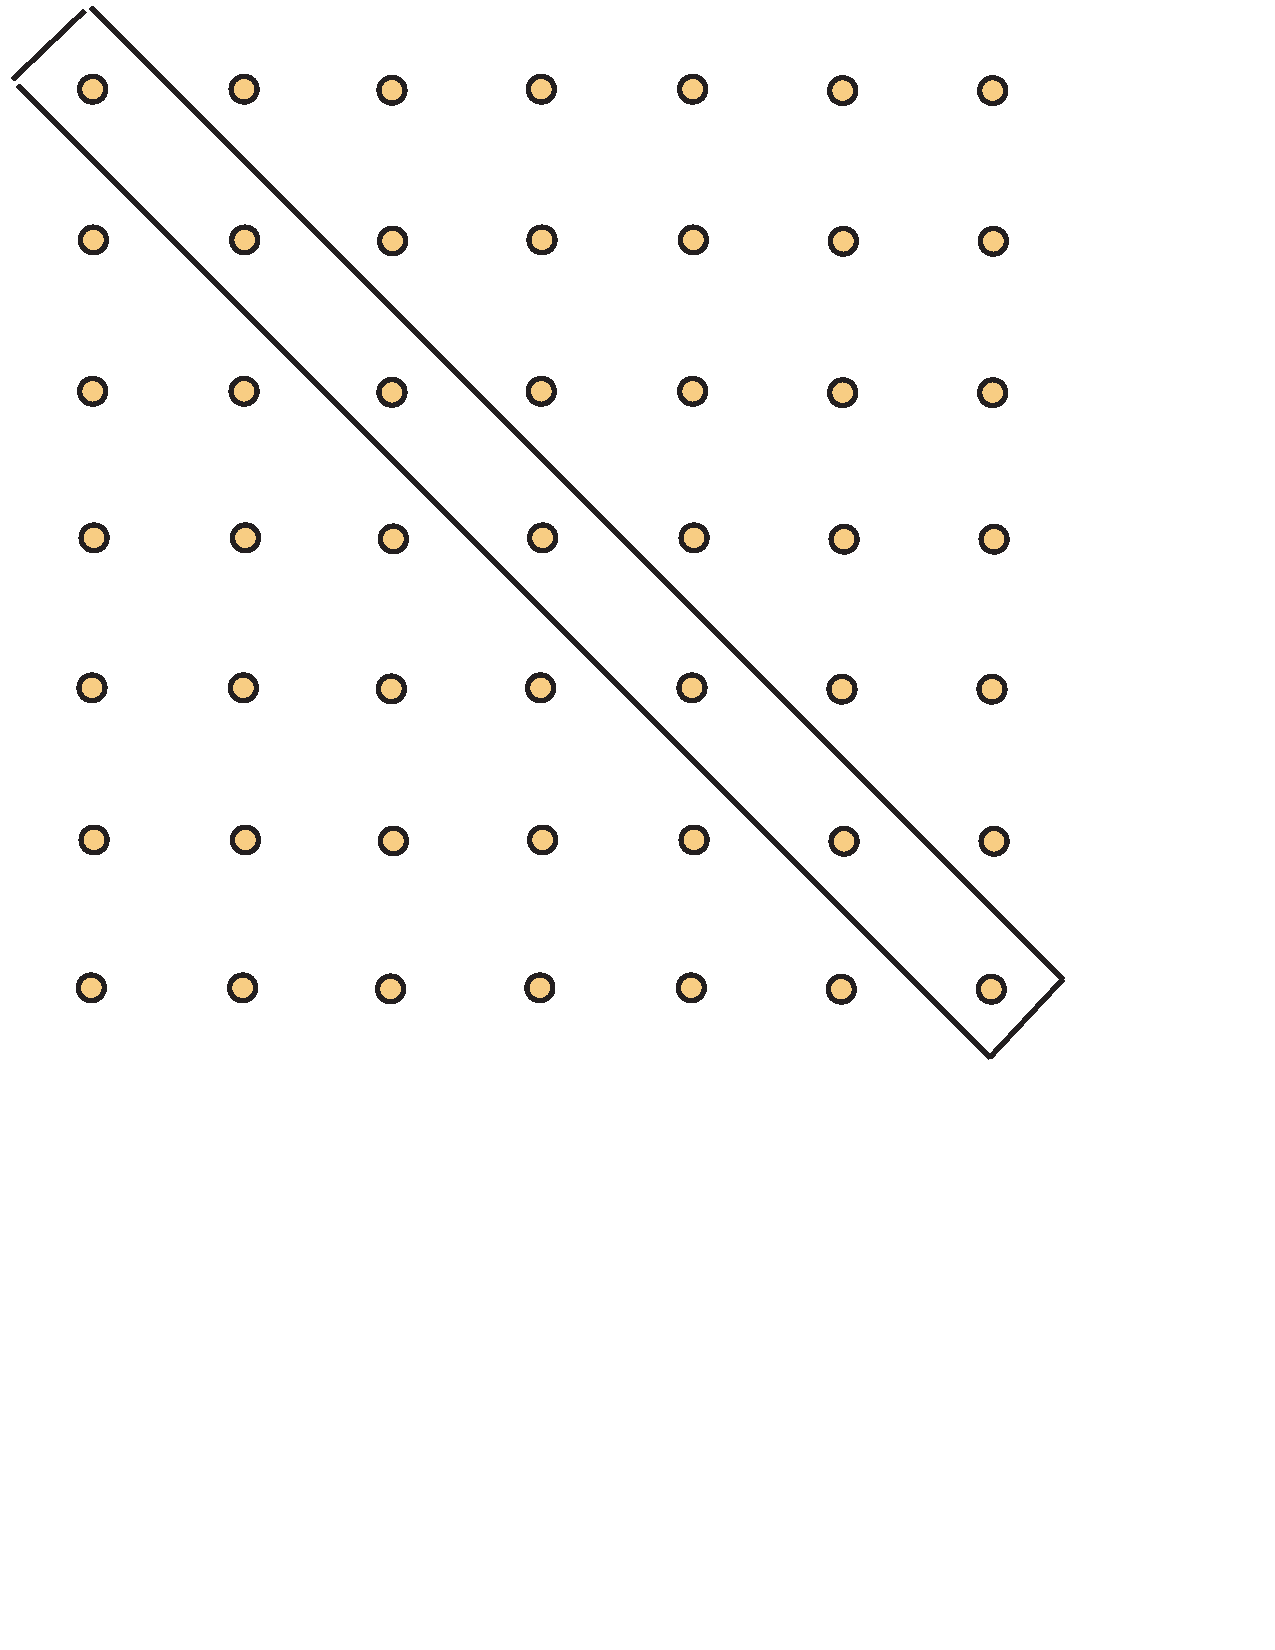
\includegraphics[viewport=0 280 516 792,scale=.3]{string-figs/3012-fig25}\\
\caption{The sum of the first $n$ integers}
\label{fig:squaredots}
\end{center}
\end{figure}


\begin{example}
Let $n$ be a positive integer. Explain why
\[
1+3+5+\dots+2n-1=n^2.
\]

The left hand side is just the
sum of the first $n$ odd integers.  But as suggested in
\autoref{fig:oddsum2}, this is clearly equal to $n^2$.

\begin{figure}
\begin{center}
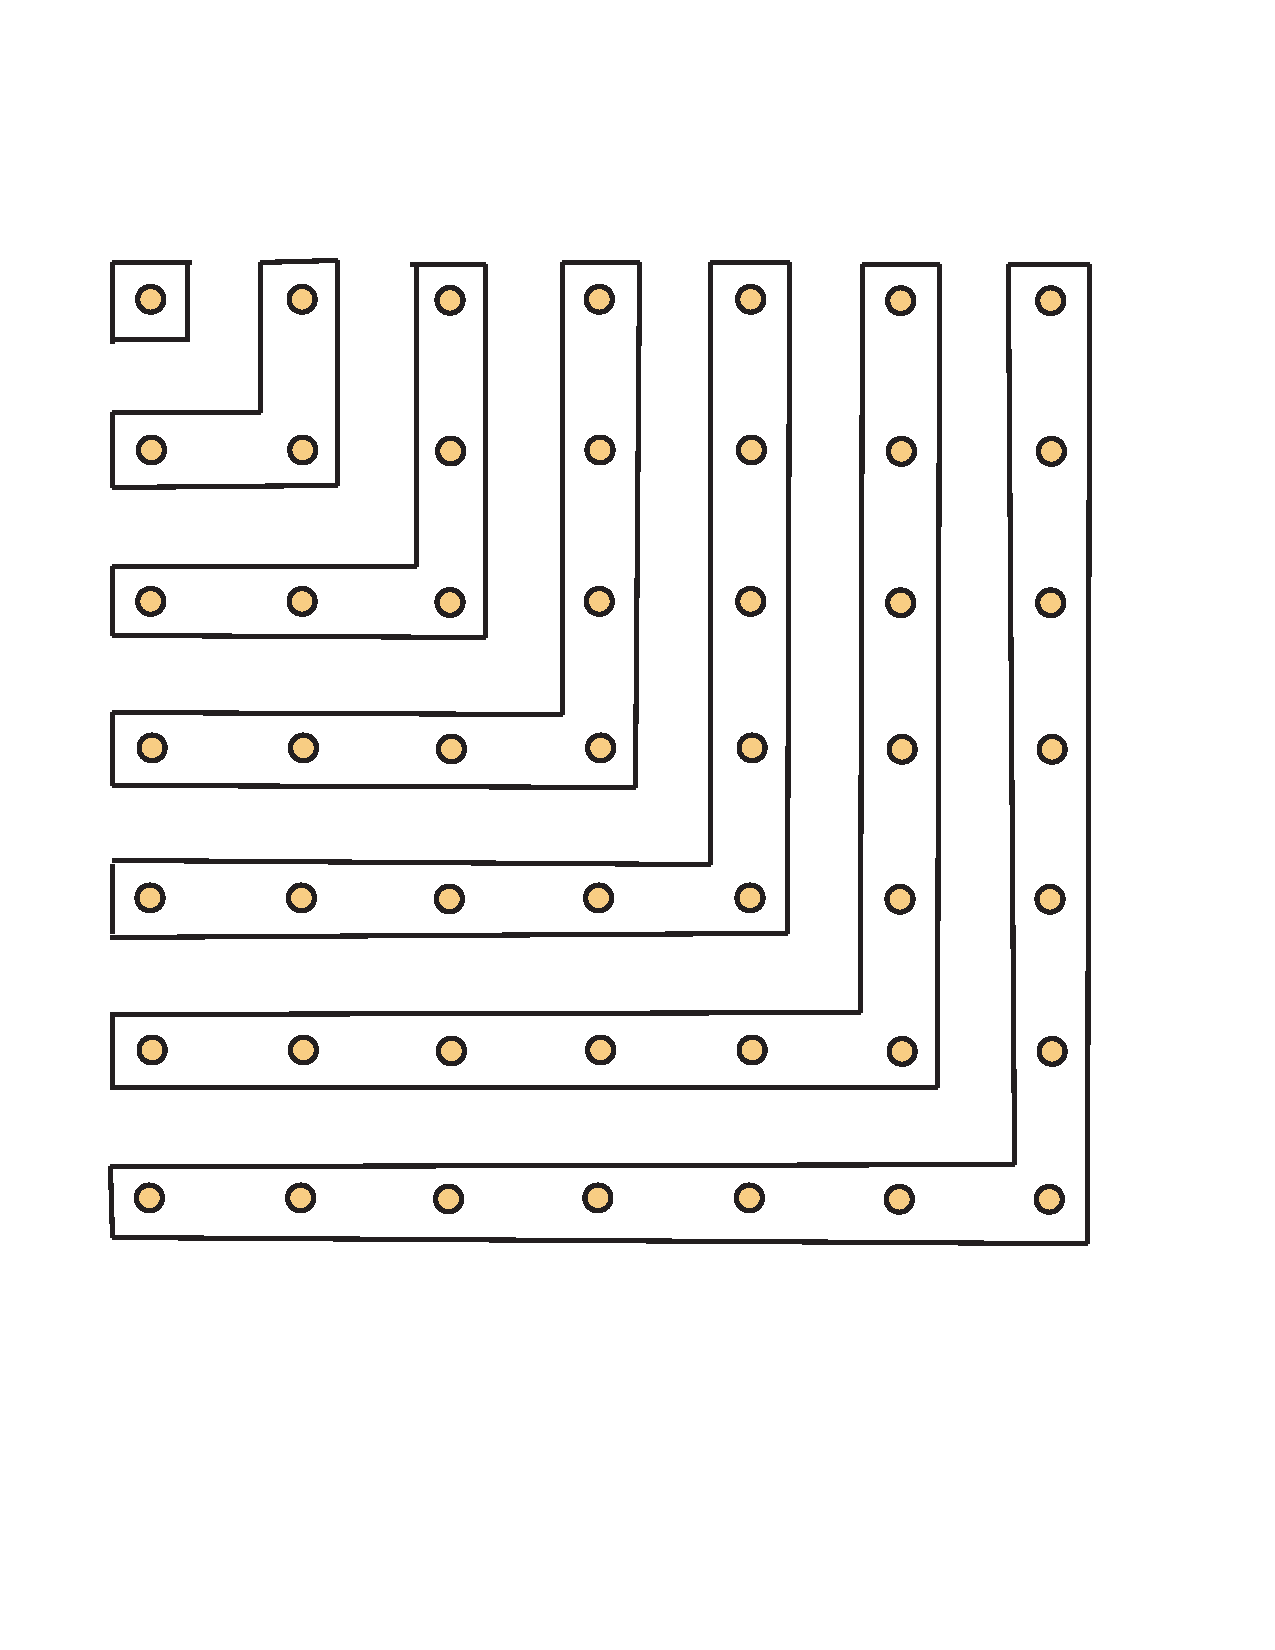
\includegraphics[viewport=45 188 534 673,scale=.3]{string-figs/3012-fig21}\\
\caption{The sum of the first $n$ odd integers
\label{fig:oddsum2}}
\end{center}
\end{figure}

\end{example}

\begin{example}
Let $n$ be a positive integer.  Explain why
\[
\binom{n}{0}+\binom{n}{1}+\binom{n}{2}+\dots+\binom{n}{n}=2^n.
\]
Both sides count the number of bit strings of length $n$, with
the left side first grouping them according to the number of
$0$'s.
\end{example}

\begin{example}
Let $n$ and $k$ be integers with $0\le k<n$.
Then
\[
\binom{n}{k+1} = \binom{k}{k} + \binom{k+1}{k} +
\binom{k+2}{k} +\dots+
\binom{n-1}{k}.
\]
To prove this formula, we simply observe that both sides count the
number of bit strings of length~$n$ that contain $k+1$ $1$'s with the
right hand side first partitioning them according to the last
occurence of a~$1$. (For example, if the last $1$ occurs in position
$k+5$, then the remaining $k$ $1$'s must appear in the preceding $k+4$
positions, giving $C(k+4,k)$ strings of this type.)  Note that
when $k=1$ (so $k+1=2$), we have the same formula as developed earlier for the
sum of the first $n$ positive integers.
\end{example}

\begin{example}
Explain the identity
\[3^n=\binom{n}{0}2^0+\binom{n}{1}2^1+\binom{n}{2}2^2+
\dots+\binom{n}{n}2^n.
\]
Both sides count the number of $\{0,1,2\}$-strings of length~$n$,
the right hand side first partitioning them according to positions
in the string which are not~$2$. (For instance, if $6$ of the
positions are not~$2$, we must first choose those $6$ positions in
$C(n,6)$ ways and then there are $2^6$ ways to fill in those six
positions by choosing either a $0$ or a $1$ for each position.)
\end{example}

\begin{example}
For each non-negative integer~$n$,
\[
\binom{2n}{n}=
{\binom{n}{0}}^2+{\binom{n}{1}}^2+{\binom{n}{2}}^2+\dots+
 {\binom{n}{n}}^2.
\]
Both sides count the number of bit strings of length $2n$ with half
the bits being $0$'s, with the right side first partitioning them
according to the number of $1$'s occurring in the first $n$ positions
of the string.  Note that we are also using the trivial identity
$\binom{n}{k}=\binom{n}{n-k}$.
\end{example}

\section{The Ubiquitous Nature of Binomial Coefficients}\label{s:strings:bin-coeff}

In this section, we present several combinatorial problems
that can be solved by appeal to binomial coefficients,
even though at first glance, they do not appear to have
anything to do with sets.

\begin{example} 
  The office assistant is distributing supplies.  In how many ways can
  he distribute 18 identical folders among four office employees:
  Audrey, Bart, Cecilia and Darren, with the additional restriction that
  each will receive at least one folder?

  Imagine the folders placed in a row.  Then there are 17 gaps between
  them.  Of these gaps, choose three and place a divider in each.
  Then this choice divides the folders into four non-empty sets.  The
  first goes to Audrey, the second to Bart, etc.  Thus the answer is
  $C(17,3)$.  In Figure~\ref{fig:distrib}, we illustrate this scheme
  with Audrey receiving~$6$ folders, Bart getting~$1$, Cecilia~$4$ and
  Darren~7.

\begin{figure}
\begin{center}
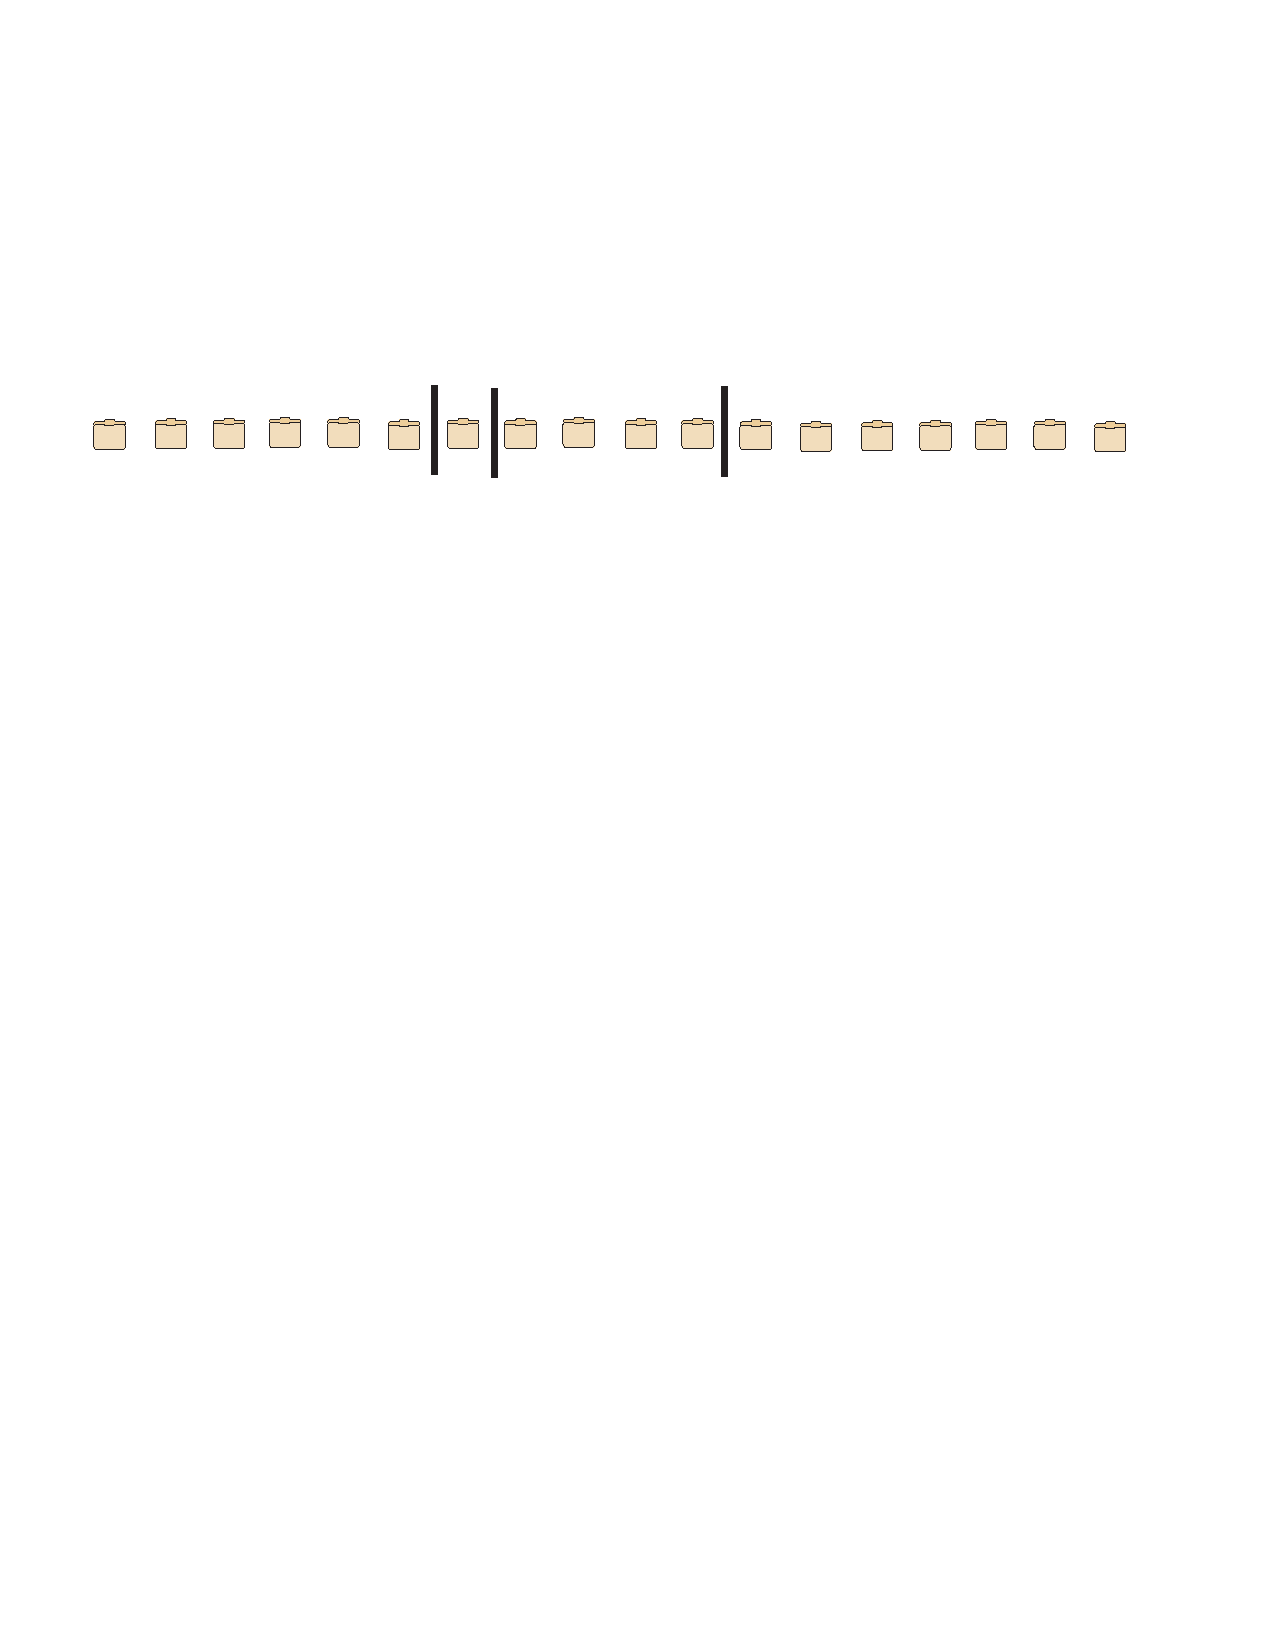
\includegraphics[viewport=36 562 544 612,scale=.6]{string-figs/3012-fig23}
\caption{{Distributing Identical Objects into Distinct
    Cells}}
\label{fig:distrib}
\end{center}
\end{figure}
\end{example}

\begin{example}
Suppose we redo the preceding problem but drop the restriction
that each of the four employees gets at least one folder.  
Now how many ways can the distribution be made?

The solution involves a ``trick'' of sorts.  First, we convert the
problem to one that we already know how to solve.  This is
accomplished by \textit{artificially} inflating everyone's allocation
by one.  In other words, if Bart will get $7$ folders, we say that he
will get $8$.  Also, artificially inflate the number of folders by
$4$, one for each of the four persons.  So now imagine a row of
$22=18+4$ folders.  Again, choose $3$ gaps.  This determines a
non-zero allocation for each person.  The actual allocation is one
less---and may be zero.  So the answer is $C(21,3)$.
\end{example}

\begin{example}
  Again we have the same problem as before, but now we want to count
  the number of distributions where only Audrey and Cecilia are
  guaranteed to get a folder. Bart and Darren are allowed to get zero
  folders.  Now the trick is to artificially inflate Bart and Darren's
  allocation, but leave the numbers for Audrey and Cecilia as is.  So
  the answer is $C(19,3)$.
\end{example}

\begin{example}
Here is a reformulation of the preceding discussion expressed in terms
of integer solutions of inequalities.

We count the number of integer solutions to the inequality
\[
x_1+x_2+x_3+x_4+x_5+x_6\le 538
\]
subject to various sets of restrictions on the values of
$x_1,x_2,\dots,x_6$.  Some of these restrictions will require
that the inequality actually be an equation.
 
The number of integer solutions is:

\begin{enumerate}
\item $C(537,5)$, when all $x_i> 0$ and equality holds.
\item $C(543,5)$, when all $x_i\ge 0$ and equality holds.
\item $C(291,3)$, when $x_1,x_2,x_4,x_6>0$, $x_3=52$,
$x_5=194$, and equality holds.
\item $C(537,6)$, when all $x_i > 0$ and the inequality is
strict. \textit{Hint:} Imagine a new variable $x_7$ which is
the balance.  Note that $x_7$ must be positive.
\item $C(543,6)$, when all $x_i \ge 0$ and the inequality is
strict. \textit{Hint:} Add a new variable $x_7$ as above.   Now it
is the only one which is required to be positive.
\item $C(544,6)$, when all $x_i \ge 0$.
\end{enumerate}
\end{example}

A classical enumeration problem (with connections to several problems)
involves counting lattice paths. A \textit{lattice path} in the plane
is a sequence of ordered pairs of integers:
\[
(m_1,n_1), (m_2,n_2), (m_3,n_3),\dots,(m_t,n_t)
\]
so that for all $i=1,2,\dots,t-1$, either
\begin{enumerate}
\item  $m_{i+1}=m_{i}+1$ and $n_{i+1}=n_i$, or
\item  $m_{i+1}=m_i$ and $n_{i+1}=n_{i}+1$.
\end{enumerate}

In Figure~\ref{fig:latticepath}, we show a lattice path from
$(0,0)$ to $(13,8)$.

\begin{figure}
\begin{center}
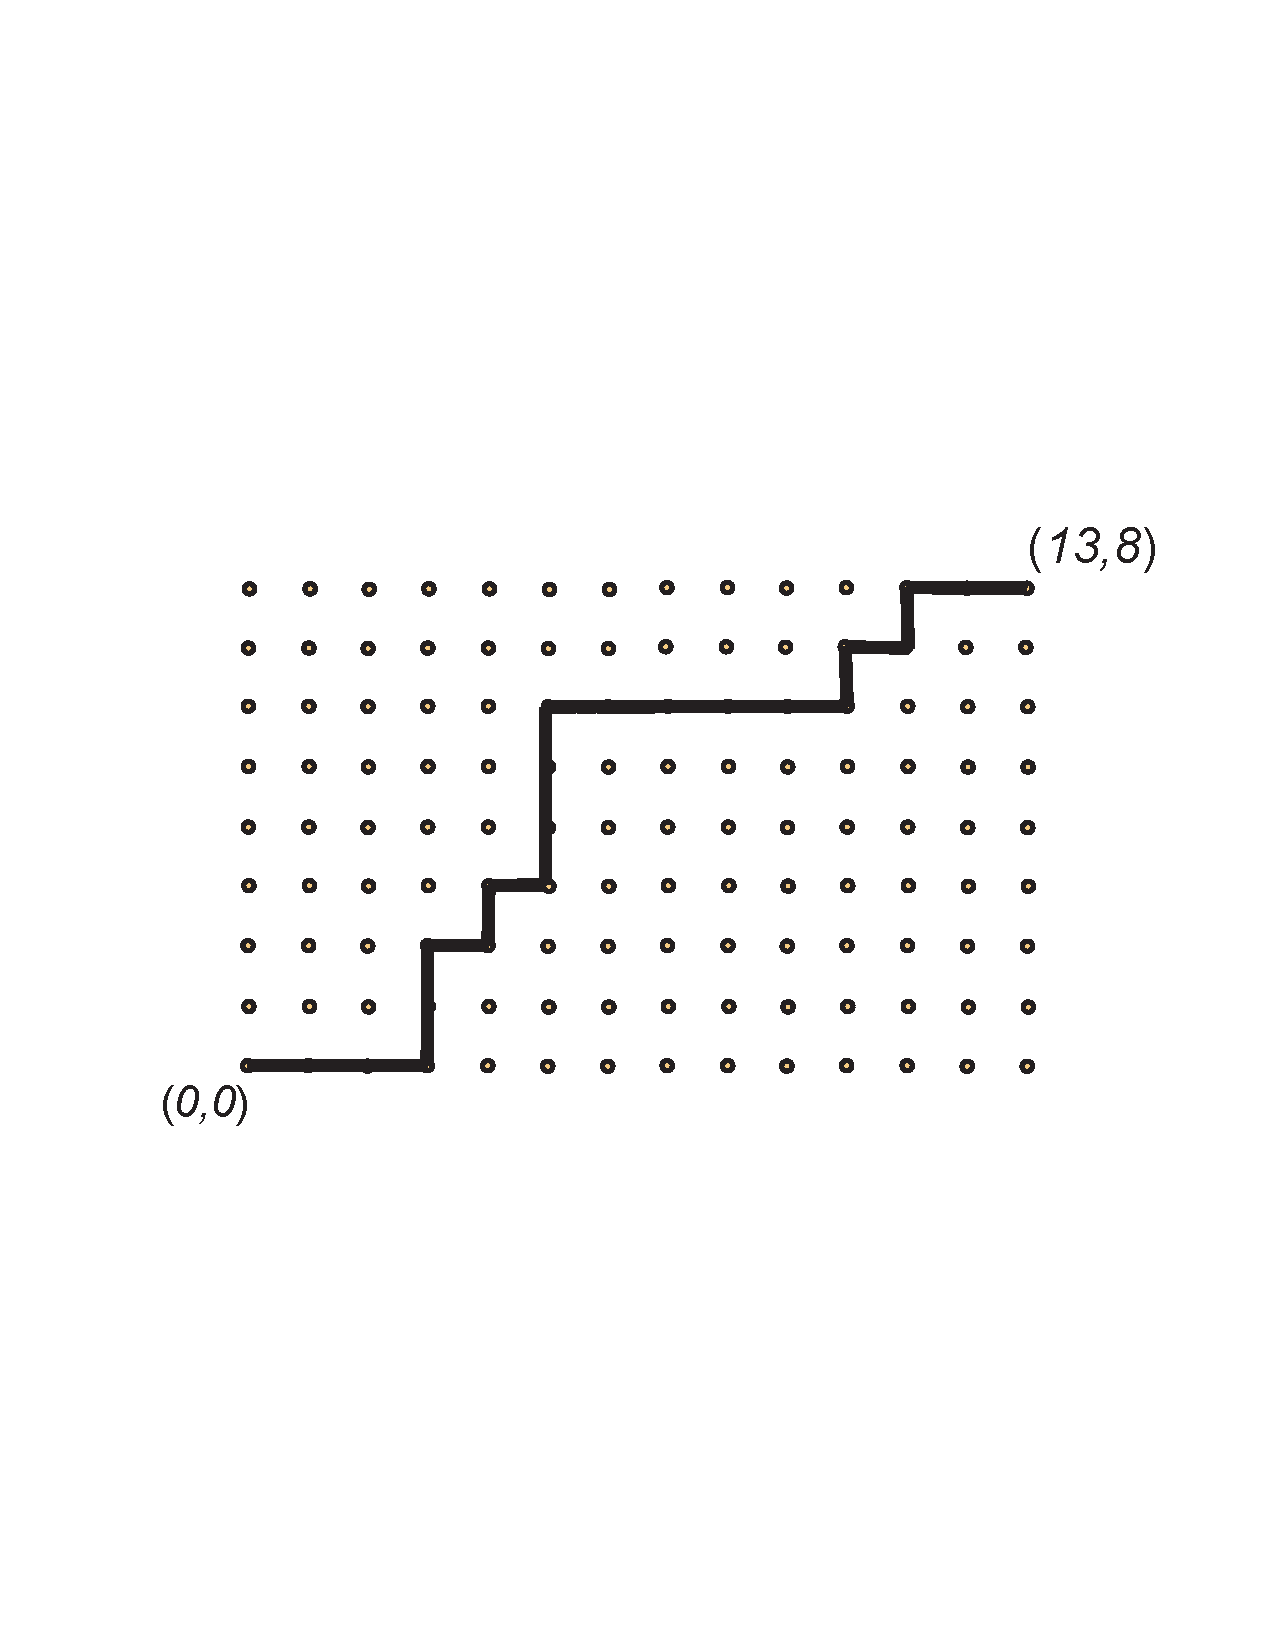
\includegraphics[viewport=72 252 552 540,scale=.4]{string-figs/3012-fig22}
\caption{A Lattice Path}
\label{fig:latticepath}
\end{center}
\end{figure}

\begin{example}  The number of lattice paths from $(m,n)$ to
$(p,q)$ is $C((p-m)+(q-n),p-m)$.

To see why this formula is valid, note that a lattice 
path is just an $X$-string with
$X=\{H,V\}$, where $H$ stands for \textit{horizontal} and $V$ stands
for \textit{vertical}.  In this case, there are exactly $(p-m)+(q-n)$
moves, of which $p-m$ are horizontal.
\end{example}

\begin{example}

Let $n$ be a non-negative integer.  Then the number of lattice
paths from $(0,0)$ to $(n,n)$ which never go above the diagonal
line $y=x$ is the Catalan number 
\[
C(n) =\frac{1}{n+1}\binom{2n}{n}.
\]

To see that this formula holds, consider the family $\cgP$ of all
lattice paths from $(0,0)$ to $(n,n)$.  A lattice path from $(0,0)$ to
$(n,n)$ is just a $\{H,V\}$-string of length $2n$ with exactly $n$
$H$'s.  So $|\cgP|=\binom{2n}{n}$.  We classify the paths in $\cgP$ as
\textit{good} if they never go over the diagonal; otherwise, they are
\textit{bad}.  A string $s\in\cgP$ is good if the number of $V$'s in
an initial segment of $s$ never exceeds the number of $H$'s.  For
example, the string ``$HHVHVVHHHVHVVV$'' is a good lattice path from
$(0,0)$ to $(7,7)$, while the path ``$HVHVHHVVVHVHHV$'' is bad.  In
the second case, note that after~$9$ moves, we have~$5$ $V$'s
and~$4$~$H$'s.

Let $\cgG$ and $\cgB$ denote the family of all good and bad paths,
respectively.  Of course, our goal is to determine $|\cgG|$.

Consider a path $s\in\cgB$. Then there is a least integer $i$ so that
$s$ has more $V$'s than $H$'s in the first $i$ positions. By the
minimality of $i$, it is easy to see that $i$ must be odd (otherwise,
we can back up a step), and if we set $i=2j+1$, then in the first
$2j+1$ positions of $s$, there are exactly $j$ $H$'s and $j+1$
$V$'s. The remaining $2n-2j-1$ positions (the ``tail of $s$'') have
$n-j$ $H$'s and $n-j-1$ $V$'s. We now transform $s$ to a new string
$s'$ by replacing the $H$'s in the tail of $s$ by $V$'s and the $V$'s
in the tail of $s$ by $H$'s and leaving the initial $2j+1$ positions
unchanged. For example, see Figure~\ref{flippath}, where the path $s$
is shown solid and $s'$ agrees with $s$ until it crosses the line
$y=x$ and then is the dashed path. Then $s'$ is a string of length
$2n$ having $(n-j)+(j+1) = n+1$ $V$'s and $(n-j-1)+j=n-1$ $H$'s, so
$s'$ is a lattice path from $(0,0)$ to $(n-1,n+1)$. Note that there
are $\binom{2n}{n-1}$ such lattice paths.

\begin{figure}
\begin{center}
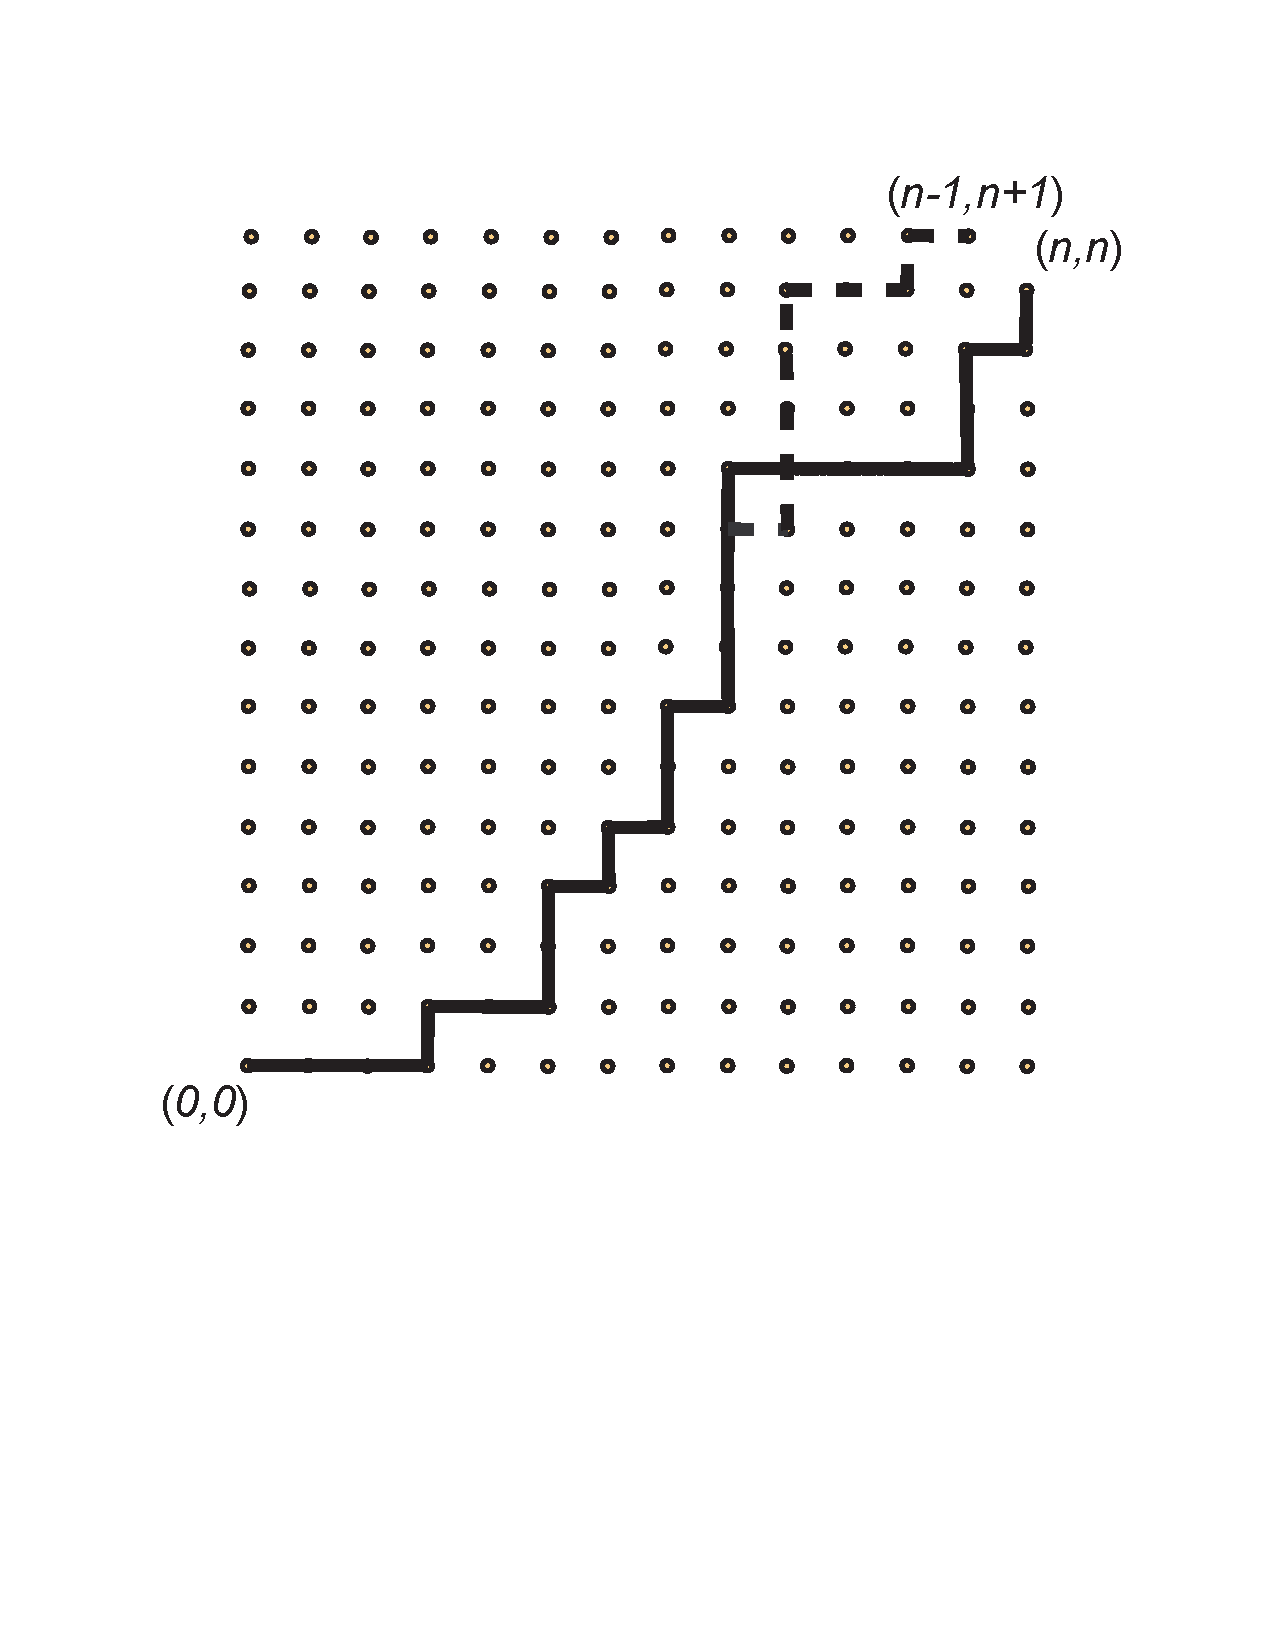
\includegraphics[viewport=69 240 550 714,scale=.4]{string-figs/3012-fig26}\\
\caption{Transforming a Lattice Path}
\label{flippath}
\end{center}
\end{figure}

We can also observe that the transformation we've described is in fact
a bijection between $\cgB$ and $\cgP'$, the set of lattice paths from
$(0,0)$ to $(n-1,n+1)$. To see that this is true, note that every path
$s'$ in $\cgP'$ must cross the line $y=x$, so there is a first time it
crosses it, say in position $i$. Again, $i$ must be odd, so $i=2j+1$
and there are $j$ $H$'s and $j+1$ $V$'s in the first $i$ positions of
$s'$. Therefore the tail of $s'$ contains $n+1-(j+1)=n-j$ $V$'s and
$(n-1)-j$ $H$'s, so interchanging $H$'s and $V$'s in the tail of $s'$
creates a new string $s$ that has $n$ $H$'s and $n$ $V$'s and thus
represents a lattice path from $(0,0)$ to $(n,n)$, but it's still a
bad lattice path, as we did not adjust the first part of the path,
which results in crossing the line $y=x$ in position $i$. Therefore,
$|\cgB|=|\cgP'|$ and thus
\[C(n)=|\cgG|=|\cgP|-|\cgB|=|\cgP|-|\cgP'| = \binom{2n}{n} -
\binom{2n}{n-1} = \frac{1}{n+1}\binom{2n}{n},\]
after a bit of algebra.
\end{example}

It is worth observing that in the preceding example, we made use of
two common enumerative techniques: giving a bijection between two
classes of objects, one of which is ``easier'' to count than the
other, and counting the objects we do \textit{not} wish to enumerate
and deducting their number from the total.

\section{The Binomial Theorem}\label{s:strings:binom-thm}

Here is a truly basic result from combinatorics kindergarten.

\begin{theorem}[Binomial Theorem]\label{thm:binomial}
Let $x$ and $y$ be real numbers with $x$, $y$ and $x+y$ non-zero.
Then for every non-negative integer $n$,
\[
(x+y)^n=\sum_{i=0}^{n}\binom{n}{i}x^{n-i}y^{i}.
\]
\end{theorem}

\begin{proof}
View $(x+y)^n$ as a product
\[ 
(x+y)^n=\underbrace{(x+y)(x+y)(x+y)(x+y)\dots(x+y)(x+y)}_{n\text{ factors}}.
\]
Each term of the expansion of the product results from choosing either
$x$ or $y$ from one of these factors.  If $x$ is chosen $n-i$ times
and $y$ is chosen $i$ times, then the resulting product is
$x^{n-i}y^i$.  Clearly, the number of such terms is $C(n,i)$, i.e.,
out of the $n$ factors, we choose the element $y$ from $i$ of them,
while we take $x$ in the remaining $n-i$.
\end{proof}

\begin{example}
  There are times when we are interested not in the full expansion of
  a power of a binomial, but just the coefficient on one of the
  terms. The Binomial Theorem gives that the coefficient of $x^5y^8$
  in $(2x-3y)^{13}$ is $\binom{13}{5}2^{5}(-3)^8$.
\end{example}

\section{Multinomial Coefficients}\label{s:strings:multinom}

Let $X$ be a set of $n$ elements.  Suppose that we have
two colors of paint, say red and blue, and we are going to
choose a subset of $k$ elements to be painted red with the
rest painted blue.  Then the number of different ways this
can be done is just the binomial coefficient $\binom{n}{k}$.
Now suppose that we have three different colors, say red,
blue, and green.  We will choose $k_1$ to be
colored red, $k_2$ to be colored blue, with the remaining
$k_3 = n - (k_1+k_2)$ colored green.  We may compute the number of
ways to do this by first choosing $k_1$ of the $n$ elements to paint
red, then from the remaining $n-k_1$ choosing $k_2$ to paint blue, and
then painting the remaining $k_3$ green. It is easy to see that 
the number of ways to do this is 
\[
\binom{n}{k_1}\binom{n-k_1}{k_2} = \frac{n!}{k_1!(n-k_1)!}
\frac{(n-k_1)!}{k_2!(n-(k_1+k_2))!} = \frac{n!}{k_1!k_2!k_3!}
\]
Numbers of this form are called \textit{multinomial coefficients};
they are an obvious generalization of the binomial coefficients.
The general notation is:

\[
\binom{n}{k_1,k_2,k_3,\dots,k_r}=\frac{n!}{k_1!k_2!k_3!\dots k_r!}.
\]
For example, 
\[
\binom{8}{3,2,1,2}=\frac{8!}{3!2!1!2!}= 
  \frac{40320}{6\cdot2\cdot1\cdot2}=1680.
\]
Note that there is some ``overkill'' in this notation, since
the value of $k_r$ is determined by $n$ and the values for
$k_1$, $k_2,\dots,k_{r-1}$.  For example, with the ordinary
binomial coeffients, we just write $\binom{8}{3}$ and not
$\binom{8}{3,5}$.

\begin{example} 
How many different rearrangements of the string:
\[
\text{MITCHELTKELLERANDWILLIAMTTROTTERAREREGENIUSES!!}
\]
are possible if all letters and characters must be used?

To answer this question, we note that there are a total of $45$
characters distributed as follows: 3~A's, 1~C, 1~D, 7~E's, 1~G, 1~H,
4~I's, 1~K, 5~L's, 2~M's, 2~N's, 1~O, 4~R's, 2~S's, 6~T's, 1~U, 1~W,
and 2~!'s.  So the number of rearrangements is
\[
\frac{45!}{3!1!1!7!1!1!4!1!5!2!2!1!4!2!6!1!1!2!}.
\]
\end{example}

Just as with binomial coefficients and the Binomial Theorem, the
multinomial coefficients arise in the expansion of powers of a
multinomial:

\begin{theorem}[Multinomial Theorem]
  Let $x_1, x_2, \dots, x_r$ be nonzero real numbers with
  $\sum_{i=1}^r x_i\neq 0$. Then for every $n\in \nni$,
  \[(x_1+x_2+\cdots + x_r)^n =
  \sum_{k_1+k_2+\cdots+k_r=n}\binom{n}{k_1,k_2,\dots,k_r}
  x_1^{k_1}x_2^{k_2}\cdots x_r^{k_r}.\]
\end{theorem}

\begin{example}
  What is the coefficient of $x^{99}y^{60}z^{14}$ in
  $(2x^3+y-z^2)^{100}$? What about $x^{99}y^{61}z^{13}$?

  By the Multinomial Theorem, the expansion of $(2x^3+y-z^2)^{100}$
  has terms of the form
  \[\binom{100}{k_1,k_2,k_3} (2x^3)^{k_1}y^{k_2}(-z^2)^{k_3} =
  \binom{100}{k_1,k_2,k_3} 2^{k_1}x^{3k_1}y^{k_2}(-1)^{k_3}z^{2k_3}.\]
  The $x^{99}y^{60}z^{14}$ arises when $k_1 = 33$, $k_2=60$, and
  $k_3=7$, so it must have coefficient
  \[-\binom{100}{33,60,7}2^{33}.\]

  For $x^{99}y^{61}z^{13}$, the exponent on $z$ is odd, which cannot
  arise in the expansion of $(2x^3+y-z^2)^{100}$, so the coefficient
  is $0$.
\end{example}

\section{Discussion}

Over coffee, Xing said that he had been experimenting with
the Maple software discussed in the introductory chapter.
He understood that Maple was treating a big integer as a string.
Xing enthusiastically reported that he had asked Maple to
find the sum $a+b$ of two large integers $a$ and $b$, each having more
than $800$ digits.  Maple found the answer about as fast as he
could hit the enter key on his netbook. 
``That's not so impressive'' Alice interjected.
``A human, even Bob, could do this in a couple of minutes using
pencil and paper.''  ``Thanks for your kind remarks,'' replied Bob,
with the rest of  the group noting that that Alice was being pretty
harsh on Bob and not for any good reason.

Dave took up Bob's case with the remark that ``Very few humans, not
even you Alice, would want to tackle finding the product of $a$ and
$b$ by hand.''  Xing jumped back in with ``That's the point.  Even
a tiny netbook can find the product very, very quickly.  In fact, I tried
it out with two integers, each having more than one thousand
digits.  It found the product in about one second.''  Ever the
skeptic, Zori said ``You mean you carefully typed in two
integers of that size?''  Xing quickly replied ``Of course not.  I
just copied and pasted the data from one source to another.''
Yolanda said ``What a neat trick that is.  Really cuts down the
chance of an error.''

Dave said ``What about factoring?  Can your netbook with its
fancy software for strings factor big integers?''  Xing
said that he would try some sample problems and report back.  
Carlos said  ``Factoring an integer with several hundred digits is
likely to be very challenging, not only for a netbook, but also for
a super computer.  For example, suppose the given integer was
either a prime or the product of two large primes.  Detecting
which of these two statements holds could be very difficult.''

Undeterred, Dave continued ''What about exponentiation?  Can your
software calculate $a^b$ when $a$ and $b$ are large integers?''
Xing said ``That shouldn't be a problem.  After all, $a^b$ is just
multiplying $a$ times itself a total of $b$ times, and if you
can do multiplication quickly, that's just a loop.''  Yolanda said
that the way Xing was describing things, he was actually
talking about a program with nested loops so it might take a long time 
for such a program to halt.  Carlos was quiet but he thought
there might be ways to speed up such computations.

By this time, Alice reinserted herself into the conversation ``Hey guys.
While you were talking, I was looking for big integer topics on the
web and found this problem.  Is $838200020310007224300$ a Catalan number?
How would you answer this?  Do you have to use special software?''

Zori was not happy.  She gloomily envisioned a future job hunt
in which she was compelled to use big integer arithmetic as a job skill.  Arrgghh.

\section{Exercises}\label{s:strings:exercises}
  \begin{enumerate}
  \item The Hawaiian alphabet consists of $12$ letters. How many
    six-character strings can be made using the Hawaiian alphabet?
  \item How many $2n$-digit positive integers can be formed if the
    digits in odd positions (counting the rightmost digit as position
    $1$) must be odd and the digits in even positions must be even and
    positive?
  \item Matt is designing a website authentication system. He knows
    passwords are most secure if they contain letters, numbers, and
    symbols. However, he doesn't quite understand that this additional
    security is defeated if he specifies in which positions each
    character type appears. He decides that valid passwords for his
    system will begin with three letters (uppercase and lowercase both
    allowed), followed by two digits, followed by one of $10$ symbols,
    followed by two uppercase letters, followed by a digit, followed
    by one of $10$ symbols. How many different passwords are there for
    his website system? How does this compare to the total number of
    strings of length $10$ made from the alphabet of all uppercase and
    lowercase English letters, decimal digits, and $10$ symbols?
  \item How many ternary strings of length $2n$ are there in which the
    zeroes appear only in odd-numbered positions?
  \item Suppose we are making license plates of the form
    $l_1l_2l_3-d_1d_2d_3$ where $l_1,l_2,l_3$ are capital letters in
    the English alphabet and $d_1,d_2,d_3$ are decimal digits (i.e.,
    in $\{0,1,2,3,4,5,6,7,8,9\}$) subject to the restriction that at
    least one digit is nonzero and at least one letter is $K$. How
    many license plates can we make?
  \item Mrs.\ Steffen's third grade class has $30$ students in it. The students
    are divided into three groups (numbered $1$, $2$, and $3$), each
    having $10$ students.
    \begin{enumerate}
    \item The students in group $1$ earned $10$ extra minutes of
      recess by winning a class competition. Before going out for
      their extra recess time, they form a single file line. In how
      many ways can they line up?
    \item When all $30$ students come in from recess together, they
      again form a single file line. However, this time the students
      are arranged so that the first student is from group $1$, the
      second from group $2$, the third from group $3$, and from there
      on, the students continue to alternate by group in this
      order. In how many ways can they line up to come in from recess?
    \end{enumerate}
  \item How many strings of the form $l_1l_2d_1d_2d_3l_3l_4d_4l_5l_6$
    are there where
    \begin{itemize}
    \item for $1\leq i\leq 6$, $l_i$ is an uppercase letter in the
      English alphabet;
    \item for $1\leq i\leq 4$, $d_i$ is a decimal digit;
    \item $l_2$ is not a vowel (i.e., $l_2\nin\{\text{A,E,I,O,U}\}$); and
    \item the digits $d_1$, $d_2$, and $d_3$ are distinct (i.e.,
      $d_1\neq d_2\neq d_3\neq d_1$).
    \end{itemize}
  \item In this exercise, we consider strings made from uppercase
    letters in the English alphabet and decimal digits. How many
    strings of length $10$ can be constructed in each of the following
    scenarios?
    \begin{enumerate}
    \item The first and last characters of the string are letters.
    \item The first character is a vowel, the second character is a
      consonant, and the last character is a digit.
    \item Vowels (not necessarily distinct) appear in the third,
      sixth, and eighth positions and no other positions.
    \item Vowels (not necessarily distinct) appear in exactly two
      positions.
    \item Precisely four characters in the string are digits and no
      digit appears more than one time.
    \end{enumerate}
  \item A database uses $20$-character strings as record
    identifiers. The valid characters in these strings are upper-case
    letters in the English alphabet and decimal digits. (Recall there
    are $26$ letters in the English alphabet and $10$ decimal digits.)
    How many valid record identifiers are possible if a valid record
    identifier must meet \emph{all} of the following criteria:
    \begin{itemize}
    \item Letter(s) from the set $\{A,E,I,O,U\}$ occur in
      \emph{exactly} three positions of the string.
    \item The last three characters in the string are \emph{distinct}
      decimal digits that do not appear elsewhere in the string.
    \item The remaining characters of the string may be filled with
      any of the remaining letters or decimal digits.
    \end{itemize}
  \item Let $X$ be the set of the $26$ lowercase English letters and
    $10$ decimal digits. How many $X$-strings of length $15$
    satisfy \emph{all} of the following properties (at the same time)?
    \begin{itemize}
    \item The first and last symbols of the string are distinct digits
      (which may appear elsewhere in the string).
    \item Precisely four of the symbols in the string are the letter '$t$'.
    \item Precisely three characters in the string are elements of the
      set $V=\{a,e,i,o,u\}$ and these characters are all distinct.
    \end{itemize}
  \item A donut shop sells 12 types of donuts. A manager wants to buy
    six donuts, one each for himself and his five employees.
    \begin{enumerate}
    \item Suppose that he does this by selecting a specific type of
      donut for each person. (He can select the same type of donut for
      more than one person.) In how many ways can he do this?
    \item How many ways could he select the donuts if he wants to
      ensure that he chooses a different type of donut for each
      person?
    \item Suppose instead that he wishes to select one donut of each
      of six \emph{different} types and place them in the
      breakroom. In how many ways can he do this? (The order of the
      donuts in the box is irrelevant.)
    \end{enumerate}
  \item The sport of korfball is played by teams of eight
    players. Each team has four men and four women on it. Halliday
    High School has seven men and $11$ women interested in playing
    korfball. In how many ways can they form a korfball team from their
    18 interested students?
  \item Twenty students compete in a programming competition in which
    the top four students are recognized with trophies for first,
    second, third, and fourth places.
    \begin{enumerate}
    \item How many different outcomes are there for the top four
      places?
    \item At the last minute, the judges decide that they will award
      honorable mention certificates to four individuals who did not
      receive trophies. In how many ways can the honorable mention
      recipients be selected (after the top four places have been
      determined)? How many total outcomes (trophies plus
      certificates) are there then?
    \end{enumerate}
  \item An ice cream shop has a special on banana splits, and Xing is
    taking advantage of it. He's astounded at all the options he has
    in constructing his banana split:
    \begin{itemize}
    \item He must choose three different flavors of ice cream to place
      in the asymmetric bowl the banana split is served in. The shop
      has 20 flavors of ice cream available.
    \item Each scoop of ice cream must be topped by a sauce, chosen
      from six different options. Xing is free to put the same type of
      sauce on more than one scoop of ice cream.
    \item There are $10$ sprinkled toppings available, and he must
      choose three of them to have sprinkled over the entire banana
      split.
    \end{itemize}
    \begin{enumerate}
    \item How many different ways are there for Xing to construct a
      banana split at this ice cream shop?
    \item Suppose that instead of requiring that Xing choose exactly
      three sprinkled toppings, he is allowed to choose between zero
      and three sprinkled toppings. In this scenario, how many
      different ways are there for him to construct a banana split?
    \end{enumerate}
 \item Suppose that a teacher wishes to distribute $25$ identical
    pencils to Ahmed, Barbara, Casper, and Dieter such that Ahmed and
    Dieter receive at least one pencil each, Casper receives no more
    than five pencils, and Barbara receives at least four pencils. In
    how many ways can such a distribution be made?
  \item How many integer-valued solutions are there to each of the
    following equations and inequalities?
    \begin{enumerate}
    \item $x_1+x_2+x_3+x_4+x_5=63$, all $x_i>0$
    \item $x_1+x_2+x_3+x_4+x_5=63$, all $x_i\geq 0$
    \item $x_1+x_2+x_3+x_4+x_5\leq 63$, all $x_i\geq 0$
    \item $x_1+x_2+x_3+x_4+x_5=63$, all $x_i\geq 0$, $x_2\geq 10$
    \item $x_1+x_2+x_3+x_4+x_5=63$, all $x_i\geq 0$, $x_2\leq 9$
    \end{enumerate}
  \item How many integer solutions are there to the equation
    \[x_1+x_2+x_3+x_4 = 132\]
    provided that $x_1>0$, and $x_2,x_3,x_4\geq 0$? What if we add the
    restriction that $x_4<17$?
  \item How many integer solutions are there to the inequality
    \[x_1+x_2+x_3+x_4+x_5\leq 782\] provided that
    $x_1,x_2>0$, $x_3\geq 0$, and $x_4,x_5\geq 10$?
  \item A teacher has $450$ identical pieces of candy. He wants to
    distribute them to his class of $65$ students, although he is
    willing to take some leftover candy home. (He does not insist on
    taking any candy home, however.) The student who won a contest in
    the last class is to receive at least $10$ pieces of candy as a
    reward. Of the remaining students, $34$ of them insist on
    receiving at least one piece of candy, while the remaining $30$
    students are willing to receive no candy.
    \begin{enumerate}
    \item In how many ways can he distribute the candy?
    \item In how many ways can he distribute the candy if, in addition
      to the conditions above, one of his students is diabetic and can
      receive at most $7$ pieces of candy?  (This student is one of
      the $34$ who insist on receiving at least one piece of candy.)
   \end{enumerate}
  \item Give a combinatorial argument to prove the identity
    \[k\binom{n}{k} = n\binom{n-1}{k-1}.\] \textit{Hint}: Think of
    choosing a team with a captain.
  \item Let $m$ and $w$ be positive integers. Give a combinatorial
    argument to prove that for integers $k\geq 0$,
    \[\sum_{j=0}^k \binom{m}{j}\binom{w}{k-j} = \binom{m+w}{k}.\]
  \item How many lattice paths are there from $(0,0)$ to $(10,12)$?
  \item How many lattice paths are there from $(3,5)$ to $(10,12)$?
  \item How many lattice paths are there from $(0,0)$ to $(10,12)$
    that pass through $(3,5)$?
  \item How many lattice paths from $(0,0)$ to $(17,12)$ are there
    that pass through $(7,6)$ and $(12,9)$?
  \item How many lattice paths from $(0,0)$ to $(14,73)$ are there
    that do \textit{not} pass through $(6,37)$?
  \item A small-town bank robber is driving his getaway car from the
    bank he just robbed to his hideout. The bank is at the
    intersection of $1^\text{st}$ Street and $1^\text{st}$ Avenue. He
    needs to return to his hideout at the intersection of
    $7^\text{th}$ Street and $5^\text{th}$ Avenue. However, one of his
    lookouts has reported that the town's one police officer is parked
    at the intersection of $4^\text{th}$ Street and $4^\text{th}$
    Avenue. Assuming that the bank robber does not want to get
    arrested and drives only on streets and avenues, in how many ways
    can he safely return to his hideout?  (Streets and avenues are
    uniformly spaced and numbered consecutively in this small town.)
  \item The setting for this problem is the fictional town of
    Mascotville, which is laid out as a grid. Mascots are allowed to
    travel only on the streets, and not ``as the yellow jacket
    flies.''  Buzz, the Georgia Tech mascot, wants to go visit his
    friend Thundar, the North Dakota State University mascot, who
    lives $6$ blocks east and $7$ blocks north of Buzz's
    hive. However, Uga VIII has recently moved into the doghouse $2$
    blocks east and $3$ blocks north of Buzz's hive and already has a
    restraining order against Buzz. There's also a pair of tigers (mother
    and cub) from
    Clemson who live $1$ block east and $2$ blocks north of Uga VIII,
    and they're known for setting traps for Buzz. Buzz wants to travel
    from his hive to Thundar's pen every day without encountering Uga
    VIII or The Tiger and The Tiger Cub. However, he wants to avoid
    the boredom caused by using a route he's used in the past. What is
    the largest number of consecutive days on which Buzz can make the
    trip to visit Thundar without reusing a route (you may assume
    the routes taken by Buzz only go east and north)?
  \item Determine the coefficient on $x^{15}y^{120}z^{25}$ in
    $(2x+3y^2+z)^{100}$.
    % Answer: 2^{15}3^{60}\binom{100}{15,60,25}
  \item Determine the coefficient on $x^{12}y^{24}$ in
    $(x^3+2xy^2+y+3)^{18}$. (Be careful, as $x$ and $y$ now appear in
    multiple terms!)
  \item For each word below, determine the number of rearrangements of
    the word in which all letters must be used.
    \begin{enumerate}
    \item OVERNUMEROUSNESSES
    \item OPHTHALMOOTORHINOLARYNGOLOGY
    \item HONORIFICABILITUDINITATIBUS (the longest word in the English
      language consisting strictly of alternating consonants and vowels\footnote{\url{http://www.rinkworks.com/words/oddities.shtml}})
    \end{enumerate}
  \item How many ways are there to paint a set of $27$ elements such
    that $7$ are painted white, $6$ are painted old gold, $2$ are
    painted blue, $7$ are painted yellow, $5$ are painted green, and
    $0$ of are painted red?
  \item There are many useful sets that are enumerated by the Catalan
    numbers. (Volume two of R.P.~Stanley's \emph{Enumerative
      Combinatorics} contains a famous (or perhaps infamous) exercise
    in $66$ parts asking readers to find bijections that will show
    that the number of various combinatorial structures is $C(n)$, and
    his \href{http://www-math.mit.edu/~rstan/ec/catadd.pdf}{web page}
    boasts an additional list of at least $100$ parts.) Give bijective
    arguments to show that each class of objects below is enumerated
    by $C(n)$. (All three were selected from the list in Stanley's
    book.)
    \begin{enumerate}
    \item The number of ways to fully-parenthesize a product of $n+1$
      factors as if the ``multiplication'' operation in question were
      not necessarily associative. For example, there is one way to
      parenthesize a product of two factors $(a_1a_2)$, there are two
      ways to parenthesize a product of three factors ($(a_1(a_2a_3))$
      and $((a_1a_2)a_3)$), and there are five ways to parenthesize a
      product of four factors: \[(a_1(a_2(a_3a_4))),
      (a_1((a_2a_3)a_4)), ((a_1a_2)(a_3a_4)),
      ((a_1(a_2a_3))a_4), (((a_1a_2)a_3)a_4).\]
    \item Sequences of $n$ $1$'s and $n$ $-1$'s in which the sum of
      the first $i$ terms is nonnegative for all $i$.
    \item Sequences $1\leq a_1\leq \cdots \leq a_n$ of integers with
      $a_i\leq i$. For example, for $n=3$, the sequences are
      \[111\qquad 112\qquad 113\qquad 122\qquad 123.\] \textit{Hint}:
      Think about drawing lattice paths on paper with grid lines and
      (basically) the number of boxes below a lattice path in a
      particular column.
  \end{enumerate}

\end{enumerate}


%%% Local Variables: 
%%% mode: latex
%%% TeX-master: "chap-skel-mtk"
%%% End: 
